\section{Synthesis in Live Programming}
\label{sec:goal}


Writing a program is a relatively static process: a programmer writes some code and, after a successful compilation, can observe and inspect its behavior. If the code does not actually implement the programmer's intentions, she can correct the program and repeat the process.

The live programming paradigm advocates a more dynamic programming cycle that allows the programmer to inspect and understand the code as it is written. While existing incarnations of live programming environments mainly focus on programs with graphical output, we propose creating a general-purpose live programming framework, which is based
on the programming by example paradigm. 

Programming by example (PBE)~\cite{cypher93,lieberman01,synasc12} is a synthesis technique that automatically generates programs that coincide with given examples. An example is specified as a tuple of input and output values. Given a set $S= \{(i_1, o_1),\ldots, (i_n, o_n)\}$ of input/output examples, the goal is to automatically derive a program $P$ such that for every $j$, $P(i_j) = o_i$. The success and impact of this line of work can be estimated from the fact that some of this technology ships as part of the popular Flash Fill feature in Excel 2013~\cite{flashFillPOPL}.

Instead of writing code, the user provides a list of relevant examples and the synthesis tool automatically generates a program. In this way, the examples can be seen as an easily readable and understandable specification. However, even if the synthesized program satisfies all the provided examples, it still might not correspond to the user's intentions. Examples are, by nature, an incomplete specification. We believe that a live programming environment is an ideal framework to address this issue. Since the program continuously interacts with the programming environment, the user can provide new examples that better illustrate her intentions, and a synthesized program can be refined with each new example. We call this approach {\emph{cooperative programming}}.

Overall, our framework should incorporate programming by example technology with
Haskell. A live programming environment is obtained through a standard
Haskell REPL (Read Evaluate Print Loop) paradigm. 

\noindent\fbox{%
    \parbox{\textwidth}{%
A small demo of our envisioned approach is available in the following video \\
$\qquad$\url{https://www.youtube.com/watch?v=w5aI3N4dq2w}.    }%
}

In this paper we outline the main research topics that such framework would need to address. 

One of the major questions is how to provide the ``best'' representative examples, 
which illustrate the programmer intentions. An approach that fits nicely
in the live programming environment is that there is a list of examples automatically
generated from the already written code. We believe that a programmer gains a better understanding of her code through observing its execution on a sequence of representative inputs. Thus, we propose extending the programming environment with an interface to explore the code's execution on a set of example input-output pairs. We plan to use a symbolic execution engine to derive these examples.  While there is some existing work on symbolic execution of Haskell, we are currently developing our own symbolic execution engine~\cite{contract, HallahanTAPAS17}.  This work is motivated by the desire for a very general framework, adaptable to a variety of purposes,  that covers a wider range of Haskell than past efforts.
In addition to the examples automatically found using symbolic execution, extra examples could be optionally provided by the developer. This could be seen as an advanced debugging tool that traces execution on several values in parallel. Fig.~\ref{fig:tool} depicts a prototype user interface of such a live programming environment.

\begin{figure}[h!]
\centering
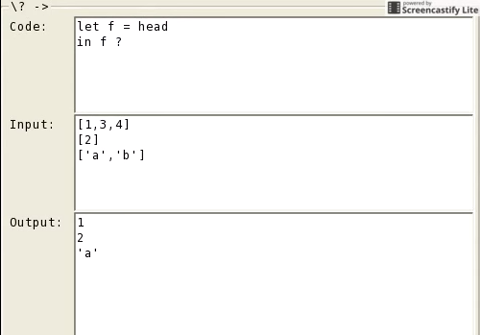
\includegraphics[scale=0.5]{tool}
\caption{A user interface for a live programming environment.}
\label{fig:tool}
\end{figure}

By observing changes in the input-output pairs, the user receives immediate feedback about whether the code is correct without actually analyzing it in detail. Any example that behaves unexpectedly acts as a real-time indication of an error in the code. 

The next question is how to correct the error? The user can go back to the code, detect
the source of the error and correct it manually. We, additionally, want to offer an 
automated repair by integrating recent advances in the PBE paradigm into this framework.
If the user notices that the current program for an input value $i$ returns an incorrect value $o$, then she can adjust that value to specify that her intended program should return $o'$ instead. This feedback could allow a tool to automatically synthesize a program which coincides with all given examples (included the modified ones) and which follows the structure of the original code as closely as possible.


\section{Research Questions Raised in Cooperative Programming }

To successfully develop the whole cooperative programming framework, 
we need to answer the following questions:
\begin{itemize}
\item How can we effectively represent the program to aid reasoning?  As previously mentioned, we plan to use symbolic execution to explore the possible inputs.  However, a major challenge here is scalability- a well known problem for symbolic execution is path explosion.  To address this, we plan to explore a variety of techniques, including aggressive identification and pruning of unhelpful paths, and making use of method summaries to abstract complicated functions.
\item Which parts of the code need to be modified so that the change is minimal with respect to some metric? In \cite{jose2011cause, pavlinovic2014finding} 
an algorithm based on MaxSAT/MaxSMT is used to find suitable candidates for the part of code in need of change. Having a representation of the code as a formula, we can apply
some of those algorithms to identify potential errors.
\item How do we efficiently produce a program from a set of examples?
%As we show in Sec.~\ref{sec:pbe} there are synthesis algorithms for some types of input/output examples. Our goal is to define a general framework for programming by example.
We plan to further study existing synthesis approaches: the current work on programming by example is focused either on type-driven synthesis, or on SAT / SMT solvers to prone the search space. We plan to investigate combination techniques, as well as entirely new algorithms for programming by example.
\item Once we have detected a source of inconsistency between the code and the given examples, and we have synthesized a correct separate code, how can we incorporate those changes so that the structure of the existing code changes as little as possible?
We have previously explored this topic in the context of firewalls~\cite{HallahanFMCAD17}.  In this work, we model firewalls as first order logic formulas, and find repairs for them, given examples of incorrectly routed packets.  We hope our experience from this work will be valuable in developing techniques for such repairs in more expressive programming languages.
%We outline our approach in Sec~\ref{sec:repair}.
\end{itemize}

We plan to extend programming-by-example technologies to fully integrate them with our live programming system. As Fig.~\ref{fig:tool} might indicate, we will develop this system in Haskell, following a long tradition of support that the Yale Computer Science Department provides for the Haskell language. To the best of our knowledge, this is the first time that these techniques will be fully integrated with a mainstream programming language.
%
%We are particularly interested in Haskell to make use of the rich type system to prune the search space more effectively. Supporting type classes, for example, would help eliminate a large class of candidates. Other GHC language extensions will be evaluated on a case-by-case basis. Some might make synthesis easier (Existential Quantification), but others might introduce significant additional complexity (Arrows, Template Haskell).

\iffalse

\subsection{Modularity}

Since our target is a real programming language, scalability plays a vital role. We therefore focus on one method of the program at a time, observe its behavior, and generate suitable examples. However, if the user wants to understand a larger logical code fragment, the examples generated for only one method will likely not illustrate the larger code's behavior well enough. By ``context'', we mean a fragment of the program that we aim to observe; when creating representative examples, the context is an important parameter.

Depending on the size of the context, parts of code in this context might need to be abstracted. The PI's ongoing work on verification of nested data structures will help in developing the right level of abstraction. In our previous work, we developed a separation-logic based tool for automated verification of linked data structures, such as lists and trees \cite{PiskacWZ14, tacasPiskacWZ14, PiskacWZ13}. When extending these results for formal verification of complex data structures, such as hash sets or B-trees (unpublished, ongoing work), we needed to abstract away certain parts once they were formally verified. We believe that applying similar abstraction techniques can help delivering more representative examples.

Haskell is a programming language with strong static typing. While Haskell's rich type system suggests a type-directed approach, the type-checking step necessitates checking all the parts of the program a given fragment references. So unless the fragment only calls code we know to be finished (not under synthesis), we cannot consider the fragment in a context isolated from the rest of the program. To address this issue, we compute method summaries, which make it easier to generate high-quality examples and to more easily correct the code. We plan to adapt an existing tool, HALO \cite{VytiniotisJCR13}, for translating Haskell programs into first-order logic formulas to use in our framework.

Type-directed synthesis is a strategy to prune the search space of candidate functions. Type-directed synthesis for simple inductively defined data types was introduced in \cite{poseraZ15}, but only leverages this simple type information. Although attempting to synthesize across the full feature-set of any modern programming language is impractical  -- C++'s template system is Turing-complete, for instance -- we believe we will be able to support at least the same subset of Haskell as HALO.
\fi
